\chapter{Communication}
\label{section:communication}

The application is web based and communicates with the server back-end over HTTP. While the client is
a complete rewrite, the server side is taken from the legacy implementation. This section discusses
the protocols and APIs involved.

Section \ref{section:commoverview} gives a conceptual overview of how the client and server talk to 
each other and exchange messages. Section \ref{section:protocol} describes the XML protocol used, 
and section \ref{section:jsrequests} deals with issuing requests from JavaScript. Finally Section
\ref{section:stores} describes how \emph{stores}, server-backed data models that support CRUD 
operations, can be used to work with items on a high level.

\section{Conceptual overview}
\label{section:commoverview}

The back-end has a pluggable architecture, with functionality divided among a set of \emph{modules}.
Each module is a named entity, such as 'maillistmodule' or 'taskitemmodule', and exposes a specific
part of the Zarafa server functionality. The client communicates with a module by sending it one or 
more \emph{actions}. Each request may contain one or mode actions for one or more modules. Several 
modules may implement the same actions (such as 'list') so actions are grouped by target module.
The server processes each of the actions in sequence and formulates a response, also containing 
actions. The process is shown in Figure \ref{figure:messageexchange}. 

Although there is usually a one-to-one mapping between response actions and request actions, this does 
not neccesarily have to hold. As an example consider the situation in Figure \ref{figure:saveitem}.
In this exchange the client wants to create a new task and sends a {\tt save} action to the
{\tt tasklistmodule} on the server, as shown in Figure \ref{figure:saveitema}. If successful, the
module on the server responds with an {\tt item} action with information about the created task, such
as the generated entry ID, but it will also send a {\tt folderupdate} action containing updated 
information about the folder the item was created in. This last action is to notify the client that
there is now one more item in the folder. 

\begin{figure}[b!]
\centering
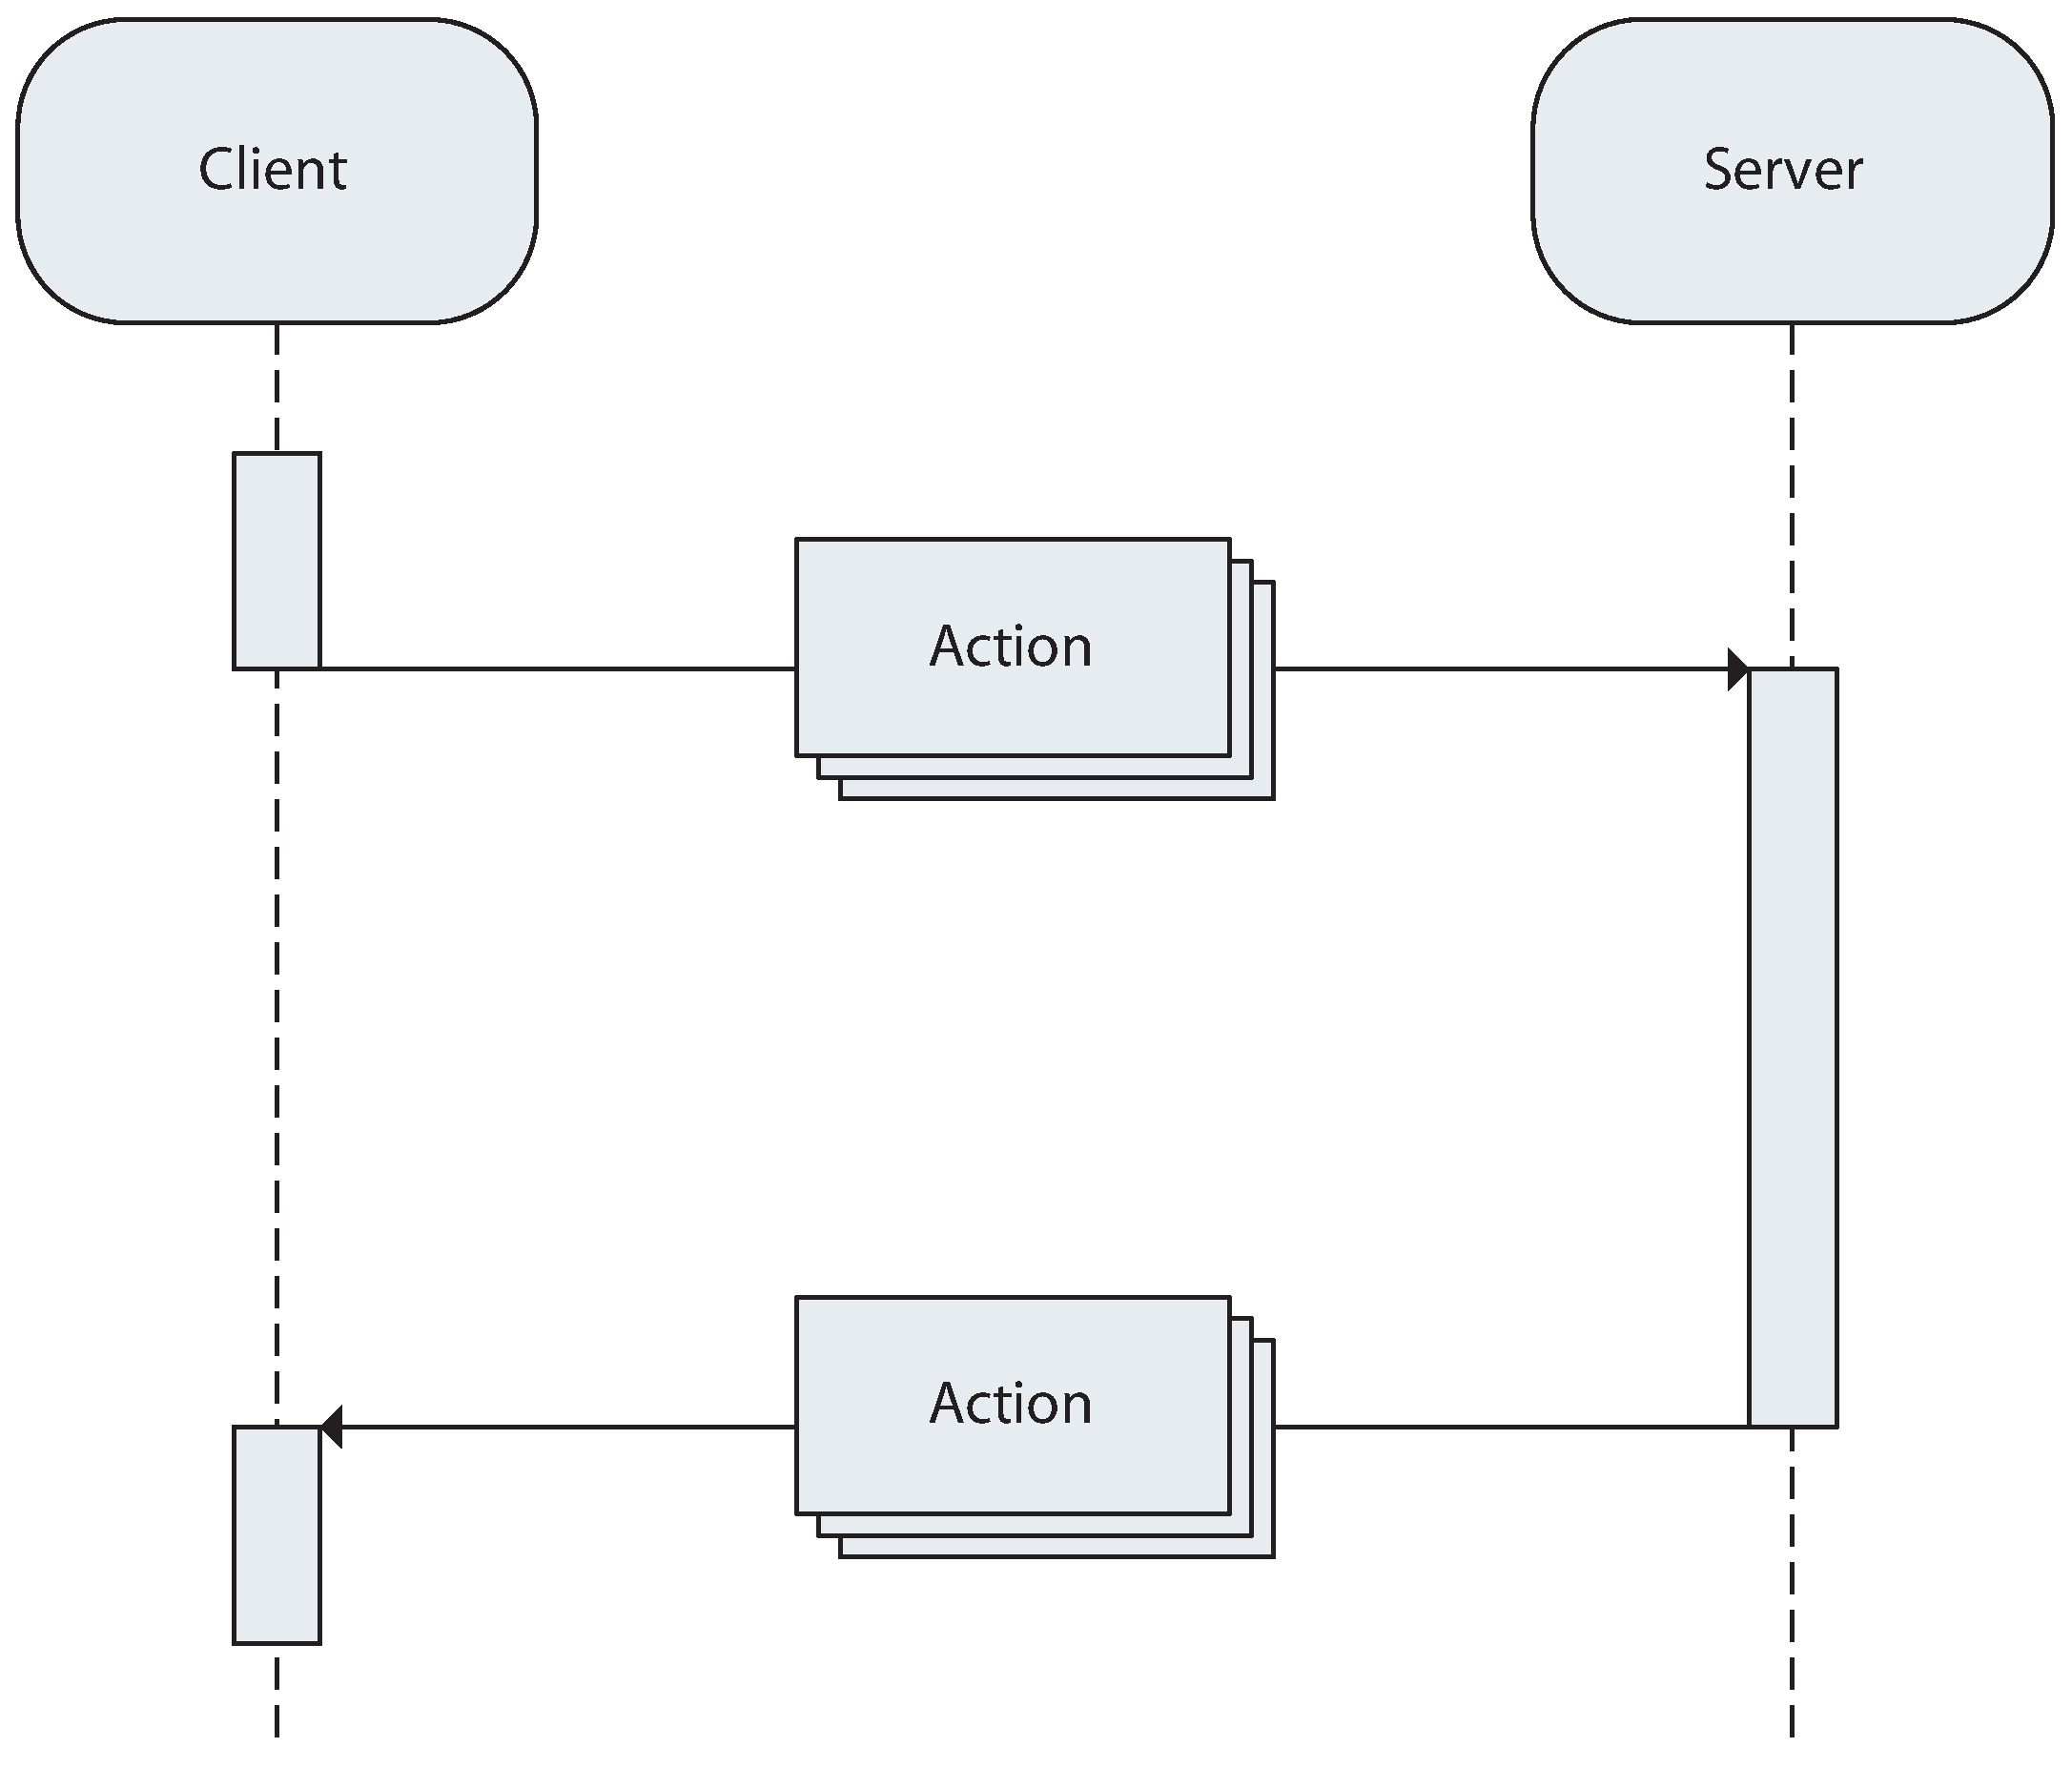
\includegraphics[width=8cm]{figures/message-exchange.eps}
\caption{A message exchange between the client and server.}
\label{figure:messageexchange}
\end{figure}

\begin{figure}
\centering
\subfigure[Client request.]
{
	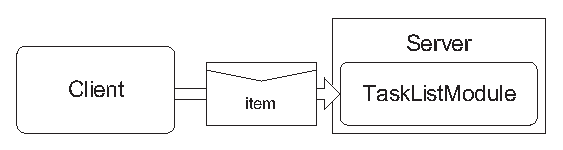
\includegraphics[width=8cm]{figures/saveitemcomm1.eps}
	\label{figure:saveitema}
}
\subfigure[Server response.]
{
	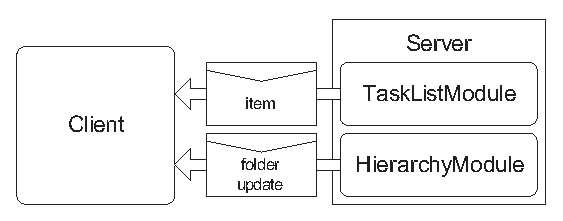
\includegraphics[width=8cm]{figures/saveitemcomm2.eps}
	\label{figure:saveitemb}
}
\caption{Message exchange for creating a new item.}
\label{figure:saveitem}
\end{figure}

\section{Protocol}
\label{section:protocol}

Communication with the back-end starts with the client initiating a request. The data exchange format is
XML. As explained in the previous section, a request may contain multiple actions for multiple modules.

\begin{lstlisting}[caption={Client server communication: client request}, label=listing:clientrequest]
<?xml version="1.0" encoding="UTF-8"?>
<zarafa>
	<module name="maillistmodule" id="maillistmodule">
		<action type="list">
			<store>[store MAPI ID]</store>
			<entryid>[folder MAPI ID]</entryid>
		</action>
	</module>
</zarafa>
\end{lstlisting}

Listing \ref{listing:clientrequest} shows a minimal client request for listing mails in a folder. Parameters
to the action are nested inside the {\tt action} tag, and may contain a forest of key-value pairs. The
server will respond with a similarly constructed reply. 

\begin{lstlisting}[caption={Client server communication: server response}, label=listing:serverresponse]
<?xml version="1.0" encoding="UTF-8"?>
<zarafa>
	<module name="previewmailitemmodule" id="previewmailitemmodule">
		<action type="item">
			[mail item details would be included here]
		</action>
	</module>
	<module name="mailnotificationmodule" id="mailnotificationmodule">
		<action type="newitem">
			[mail item details would be included here]
		</action>
	</module>
</zarafa>
\end{lstlisting}

Listing \ref{listing:serverresponse} shows a possible response from the server. Note that the behavior of 
mail notifications is currently not implemented in the legacy back-end, but that this is a definite want-to-have 
feature for the future. It is merely used as an example of how the server might send back actions that are 
not immediate responses to actions issued in the request, like in the case of Figure \ref{figure:saveitem}.

\section{Submitting requests from Javascript}
\label{section:jsrequests}

To avoid having to construct XML requests manually all client requests are made through a global instance of the
{\tt Zarafa.comm.Request} class. This object provides JavaScript$\leftrightarrow$XML (de)serialisation, and allows 
other components to react to server actions via either events or callbacks.

Consider Listing \ref{listing:request}. A call is made to the request object (a global instance of which
can be obtained from the container using {\tt getRequest()}) to retrieve a single message. The first two 
arguments are the module name and action type, which are taken from enumeration objects 
{\tt Zarafa.comm.ModuleNames} and
{\tt Zarafa.comm.Actions} respectively. The third argument is a Javascript object containing the parameters
to the action, which in this case are the message's MAPI store Id and MAPI entry Id. 

\begin{lstlisting}[caption={Submitting a request}, label=listing:request]
container.getRequest().singleRequest(

	Zarafa.comm.ModuleNames.previewReadMailItem,
	Zarafa.comm.Actions.open,
	{
		store : storeId,
		entryid : entryId
	}
);
\end{lstlisting}

The parameter object is serialised into equivalent XML and embedded into the {\tt action} xml tag. The 
serialisation can become a little involved depending on the XML you want to create. Consider the example
in Listing \ref{listing:parameters1}, and the corresponding XML in Listing \ref{listing:parameters2}

\begin{lstlisting}[caption={Parameter serialisation, JavaScript}, label=listing:parameters1]
var parameters = {
		sort : {
			column : 'date_received'
		}
};
\end{lstlisting}

\begin{lstlisting}[caption={Parameter serialisation, XML}, label=listing:parameters2]
<sort>
	<column>date_received</column>
</sort>
\end{lstlisting}

This correspondence is straightforward and easy to work with. Unfortunately 'maillistmodule' expects the
'column' node to carry an XML attribute 'direction' which should be either 'asc' or 'desc', for ascending and
descending respectively. To accomodate this an alternative form lets you specify the column tag as an
object with a {\tt \_} property for the text node, and zero or more properties starting with {\tt \$} to
describe attributes. This is exemplified in Listings \ref{listing:parameters3} and \ref{listing:parameters4}.

\begin{lstlisting}[caption={Parameter serialisation, JavaScript}, label=listing:parameters3]
var parameters = {
		sort : {
			column : {
				_ : 'date_received'
				$direction : 'desc'				
			}
		}
};
\end{lstlisting}

\begin{lstlisting}[caption={Parameter serialisation, XML}, label=listing:parameters4]
<sort>
	<column direction="desc">date_received</column>
</sort>
\end{lstlisting}

\subsection{Callbacks}

As described in the previous section there are two ways for the client to respond to server actions.
One way is to pass callback functions to the {\tt singleRequest} method. This is shown in Listing 
\ref{listing:callbacks}.

\begin{lstlisting}[caption={Using callbacks}, label=listing:callbacks]
container.getRequest().singleRequest(
	Zarafa.comm.ModuleNames.previewReadMailItem,
	Zarafa.comm.Actions.open,
	{
		store : storeId,
		entryid : entryId
	},
	{
		item : function(response)
		{
			// do something with response.data
			alert(response.data.item.body);
		},
		error : function(error)
		{
			// do something with the error
			alert(error.message);
		}
	}
);
\end{lstlisting}

In this example a Javascript object is passed as an optional fourth argument to {\tt Response.singleRequest}.
The callback argument is a key/value set with named actions linked to JavaScript functions. In our example,
if the server responds to this request with an 'item' action, the corresponding function is fired and the
mail body is displayed. Note that this function will only be called in response to an 'item' action from
the module that this request is calling (the 'previewreadmailitemmodule' in this case). The callback
will be called with a {\tt Zarafa.comm.Response} object containing a module name, action type, and a data
object which encapsulates the response data from the server.

It is also possible hook an error callback, which will be called when something goes wrong. An error
object is passed into the callback with information about the type of error and a user-friendly error 
message.

\subsection{Events}

In some cases it is in the interest of low inter-object dependency (low coupling) to have objects respond
to server actions that are not a result of a request issued directly by themselves. Consider the case
described in Section \ref{section:protocol}, where new mail notifications are piggy-backed. It is undesirable
to use callbacks to handle the 'newitem' action for two reasons. First, every request may generate such an 
action from the server, so each and every request would need to have a 'newitem' callback function attached. 
Second, callbacks are hooked by action type, and only respond to server actions from the module that the 
request was meant for. 

To address these issues the {\tt Request} object supports events that can be tied to specific combinations
of modules and actions. This makes it possible to tie a handler to the 'newitem' action of the 
'mailnotificationmodule' in any point in the code. In our example the hierarchy tree may for instance want
to listen to such events so that it may visually update the number of unread items in the user inbox.
The process is illustrated in Listing \ref{listing:events}

\begin{lstlisting}[caption={Using callbacks}, label=listing:events]
container.getRequest().addListener(
	Zarafa.comm.ModuleNames.mailNotification,
	Zarafa.comm.Actions.newItem,
	function(response)
	{
		alert('You have new mail');
	}
);
\end{lstlisting}

A special event case is the error event which, like the callback, fires when a request fails. This event
can be used to catch errors at a global scope, for instance to present the user with the opportunity
to re-login when the session has timed out.

\section{Stores}
\label{section:stores}

A MAPI folder can be seen as a flat list of items, much like a table in a database. Instead of directly issuing
action requests from the client to list or mutate items, a high-level API is provided that exposes
a MAPI folder as an ExtJS \emph{store} ({\tt Ext.data.Store}). A store is a client-side cache of items that exist
on the server, and provides a clean interface for loading and CRUD operations. 

Many standard ExtJS components use stores to manage the data they display and operate on. In MVC terms,
a store is the default \emph{model} for many UI components. A common example is the grid panel 
({\tt Ext.grid.GridPanel}). Displaying a list of tasks in a tasks folder is a matter of constructing a 
store instance, initialising it with the proper parameters (store ID), and connecting it to the grid. The
grid will automatically issue a generic 'load' command to the store to populate it with data which
is then displayed. 

\begin{figure}[t!]
\centering
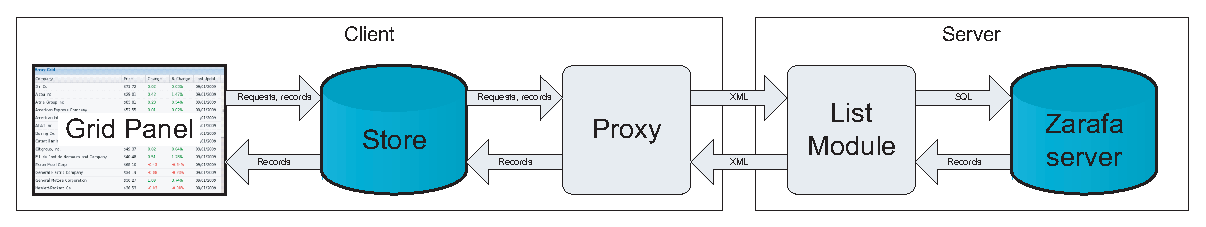
\includegraphics[width=14cm]{figures/store2.eps}
\caption{Data flow.}
\label{figure:stores}
\end{figure}

Figure \ref{figure:stores} how various components connect to get data from the server to display in a 
data grid in the browser. A grid panel is connected to a store, which acts as a local data base holding
a set of records. The store uses a proxy to talk to the server, which in turn tasks with a server-side
\emph{list module} using the communication scheme described in previous sections. The server has different 
list modules for each type of data (tasks, mail, etc), and there are corresponding stores and proxies on 
the client.

Stores can be constructed with a store- and folder MAPI id, or these can be passed explicitly to the 
load method. Please refer to Section \ref{section:taskscontext} for a code example of this principle
in action. However stores can do more than just plain data loading. They support pagination and sorting,
and it's very easy to get this to work with the standard ExtJS components.

Records can be added, removed, or updated. Changes made to the data in a store can be committed to the 
server by calling the {\tt save} method. 


